\section{Mikroprocesory}
Mikroprocesor lze definovat jako sekvenční automat vyrobený technologií VLSI (Very Large Scale Integration), což znamená, že na jednom čipu jsou integrovány obvody obsahující velké množství tranzistorů. Tato integrace umožňuje vytvoření složitých a výkonných mikroprocesorů, které jsou schopny provádět širokou škálu operací. Mikroprocesor se skládá z několika částí:
\begin{itemize}
    \item \textbf{ALU}
    \item \textbf{Registry}
        \begin{itemize}
            \item Čítač instrukcí
            \item Registr instrukce
            \item ...
        \end{itemize}
    \item \textbf{Řadič}
\end{itemize}
Mikroprocesor obsahuje další části jako například: Cache, FPU, DMA Controller, Clock Generator, Bus Interface Unit,atd..

\paragraph{Registr instrukce}
Registr instrukce slouží jako dočasná paměť pro instrukci, která se právě provádí. Obsahuje binárně zakódovanou reprezentaci aktuální instrukce, kterou mikroprocesor čte a dekóduje. Registr instrukce může být také propojen s čítačem instrukcí.

\paragraph{Čítač instrukcí}
Čítač instrukcí udržuje adresu nebo index aktuální instrukce, která se má provést. Tato adresa obvykle ukazuje na paměťovou lokaci, kde je uložen kód instrukce (binární podoba) nebo načtená instrukce přímo v paměti. Mikroprocesor pracuje sekvenčně, tj. postupuje od jedné instrukce k další podle pořadí v programu. Čítač instrukcí se aktualizuje po každé vykonané instrukci tak, aby ukazoval na následující instrukci v pořadí. Čítač instrukcí umožňuje také realizaci skoků v programu. Skoky jsou instrukce, které umožňují přeskočení na jinou adresu v programu na základě určitých podmínek (například podmíněné skoky podle výsledku porovnání).

\paragraph{Řadič}
Řadič řídí a synchronizuje činnost různých částí CPU a dalších komponent v počítači. Zajišťuje, aby se instrukce vykonávaly správně a data se přenášela mezi procesorem a pamětí nebo periferními zařízeními.  Je zodpovědný za načítání, dekódování a vykonávání instrukcí, správu dat a synchronizaci operací.

\paragraph{ALU}
ALU je jednou z nejdůležitějších komponent mikroprocesoru. Její úlohou je provádět všechny aritmetické (sčítání, odčítání, násobení, dělení) a logické operace (AND, OR, NOT) nad daty uloženými v registrech procesoru. V mnoha moderních procesorech je ALU rozdělena na více jednotek: jednu pro práci s celočíselnými operandy a další pro práci s operandy v plovoucí řadové čárce (floating-point operations). Jednotlivé ALU pracují nezávisle na sobě. Díky tomu, že jednotky ALU pracují nezávisle, procesor může zpracovávat více instrukcí současně, což zvyšuje celkovou výkonnost procesoru.

\begin{figure}[h]
    \centering
    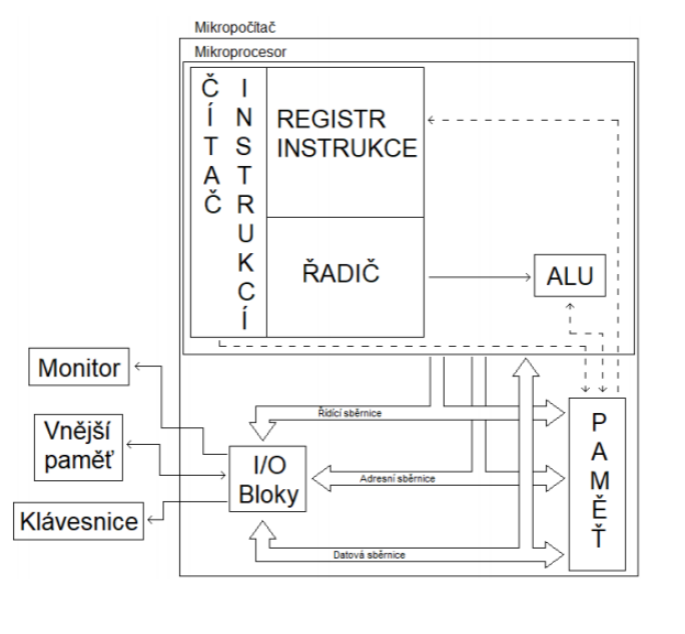
\includegraphics[width=0.5\linewidth]{sections/2_mikroprocesor/images/Screenshot 2024-08-22 133255.png}

\end{figure}

\subsection{Typy procesorů}

\subsubsection{CPU (Central Processing Unit)}
\paragraph{Popis} CPU je hlavní procesor v počítači, který provádí většinu výpočtů a řídí chod celého systému. Zpracovává instrukce z operačního systému a aplikací.
\paragraph{Použití} Všeobecné výpočty, zpracování dat, běh aplikací, řízení hardware, multitasking. 
\paragraph{Příklady} Intel Core i7, AMD Ryzen 7.

\subsubsection{GPU (Graphics Processing Unit)}
\paragraph{Popis} GPU je specializovaný procesor navržený pro rychlé vykreslování grafiky a provádění paralelních výpočtů. Má mnoho jader, která jsou schopna provádět jednoduché operace na velkém množství dat současně.
\paragraph{Použití} Vykreslování 3D grafiky, zpracování obrazu, vědecké výpočty, strojové učení, kryptoměnová těžba. 
\paragraph{Příklady} NVIDIA GeForce RTX 3080, AMD Radeon RX 6800.

\subsubsection{APU (Accelerated Processing Unit)}
\paragraph{Popis} APU je typ procesoru, který kombinuje CPU a GPU na jednom čipu. Tím se zvyšuje efektivita a snižují se náklady a spotřeba energie.
\paragraph{Použití} Levné a energeticky efektivní systémy, notebooky, počítače pro běžné použití, kde je potřeba vyvážený výkon CPU a GPU.
\paragraph{Příklady} AMD Ryzen 5 3400G, AMD A10-7850K.

\subsection{Rozdíl mezi mikroprocesorem a mikrořadičem}
\begin{center}
\begin{tabular}{|c|p{5cm}|p{5cm}|}
\hline
 & \textbf{Mikroprocesor} & \textbf{Mikrokontrolér} \\
\hline
\textbf{Konstrukce} & 
Navržen především jako výkonná centrální procesorová jednotka (CPU) s vysokou výpočetní kapacitou. Mikroprocesor je obvykle součástí komplexního systému, který zahrnuje externí paměť, vstupně-výstupní (I/O) rozhraní a další periferní zařízení. Typicky se používá ve výkonných výpočetních zařízeních, jako jsou osobní počítače, servery a mobilní telefony. & 
Integrovaný obvod, který obsahuje CPU, paměť (RAM, ROM, Flash), periferie (např. ADC, UART, GPIO) a časovač na jednom čipu. Mikrokontroléry jsou navrženy pro specifické aplikace s omezenými zdroji a jsou ideální pro řízení periferních zařízení a jednoduché úlohy. \\
\hline
\textbf{Schopnosti} & 
Nabízí vyšší výpočetní výkon a schopnost zpracovávat složité algoritmy a aplikace. & 
Nabízí nižší výkon v porovnání s mikroprocesorem, ale je dostatečný pro řízení periferií a jednoduché úlohy. \\
\hline
\textbf{Typické použití} & 
Vhodný pro aplikace vyžadující vysoký výkon, jako jsou osobní počítače, servery, mobilní zařízení a herní konzole. & 
Ideální pro aplikace vyžadující řízení a monitorování periferních zařízení, jako jsou domácí spotřebiče, automobilová elektronika, průmyslová řízení, senzory a IoT (Internet věcí). \\
\hline
\end{tabular}
\end{center}
V podstatě je mikrokontroler mikroprocesor s integrovanými periferiemi, pamětí a dalšími komponentami v jednom čipu.

\subsection{Architekrury}
\subsubsection{Instrukční sady}
\paragraph{RISC}
RISC (Reduced Instruction Set Computer) je architektura instrukční sady, která využívá menší počet jednodušších instrukcí. Cílem je dosáhnout vyšší rychlosti vykonávání díky jednodušším a rychleji vykonatelným instrukcím. RISC procesory jsou optimalizovány pro rychlé provádění těchto jednoduchých instrukcí a často používají pevnou délku instrukcí.

\paragraph{CISC}
CISC (Complex Instruction Set Computer) je architektura instrukční sady, která využívá širší spektrum komplexnějších instrukcí. Cílem je zjednodušit programování tím, že poskytuje instrukce, které mohou provádět více operací najednou. CISC procesory mají často variabilní délku instrukcí a složitější dekódování instrukcí.

\subsubsection{Fyzické architektury}

\paragraph{Harvardská architektura}
Harvardská architektura fyzicky odděluje paměť programu a dat a jejich spojovací obvody. To znamená, že instrukce a data mohou být načítány a zapisovány současně, což může zvýšit výkon systému. Harvardská architektura se často používá v DSP (Digital Signal Processing) procesorech a v některých mikrokontrolérech.

\paragraph{Von Neumannova architektura}
Von Neumannova architektura používá jednu sběrnici, na kterou jsou připojeny všechny aktivní prvky (procesor, paměť, vstupy a výstupy). Instrukce a data sdílejí stejnou paměť a sběrnici, což může vést k tomu, že se program může sám přepsat. Tato architektura je však jednodušší a levnější na implementaci a je široce používána ve většině počítačových systémů.

\subsection{Charakteristika procesoru ARM STM32F4}
STM32 je rodina 32 bitových mikrořadičů integrovaných obvodů od STMicroelectronics. Každý mikroprocesor se skládá z procesorového jádra, statické paměti RAM a flash paměti. Procesory ARM obsahují moderní vývojové prostředí a díky podpoře jazyka C i snadné programování.

\subsubsection{Specifikace}
\begin{itemize}
    \item Založen na vysoce výkonném 32 bitovém jádru RISC Cortex M4 pracujícím s frekvencí až 168 MHz
    \begin{itemize}
        \item Podporuje všechny instrukce a datové typy s jednorozměrným zpracováním dat
        \item Implementuje kompletní sadu instrukcí DSP a jednotku ochrany paměti, která zvyšuje bezpečnost
    \end{itemize}
    \item STM32 běží na 2-3,6V
    \item Paměť flash o kapacitě 1 MB a paměť RAM o kapacitě 192 kB, která je teoreticky rozšiřitelná až na 4 GB
    \item Load/Store architektura
    \begin{itemize}
        \item S pamětí pracují pouze instrukce typu load a store
        \item Všechny ostatní instrukce pracují s vnitřními registry
        \item Rozdělení na dvě kategorie (práce s pamětí a práce s registry)
    \end{itemize}
\end{itemize}

\subsubsection{Sběrnice}

\paragraph{AHB} Advanced High Performance Bus je určen pro velmi rychlou komunikaci mezi CPU, RAM a DMA. Podporuje dávkový přenos dat a slouží jako most pro komunikaci s APB.

\paragraph{APB} Advanced Peripheral Bus poskytuje jednoduché rozhraní pro připojení pomalejších a low-power periferií k CPU, jako jsou časovače, UART, I2C a SPI. Periferie komunikují s CPU prostřednictvím mostu mezi AHB a APB.

\paragraph{RCC $->$ AHB1ENR}
Registry v RCC slouží k aktivaci příslušného portu na sběrnici AHB.

\paragraph{Registry GPIOx}
GPIOx registery, jako je \texttt{MODER}, slouží k nastavení módu pinů (vstupní, výstupní) pro GPIO port x.

\paragraph{GPIOx $->$ IDR a ODR}
\texttt{IDR} (Input Data Register) umožňuje čtení stavu vstupních pinů (např. tlačítek) u GPIO portu x. Naopak \texttt{ODR} (Output Data Register) umožňuje nastavovat stav výstupních pinů (např. LED) u GPIO portu x.

\subsection{Přerušovací systémy}
Přerušovací systémy jsou základním mechanismem operačních systémů pro správu událostí a respektování priorizace různých úloh. Když se vyskytne událost (jako je například dokončení operace vstupu/výstupu, časovač, apod.), hardware může vyvolat přerušení, což je signál operačnímu systému, že něco vyžaduje jeho pozornost. Existují dva hlavní přístupy k obsluze přerušení: metoda polling a metoda interrupt.

\ToDo

\paragraph{Metoda Polling}
Metoda polling (dotazování) je jednoduchá technika, při které operační systém opakovaně (periodicky) dotazuje hardware, zda se nějaká událost stala. Například při čtení dat z periferního zařízení operační systém pravidelně kontroluje (dotazuje se), zda jsou data připravena k přenosu. Tento přístup má několik nevýhod:
\begin{itemize}
    \item \textbf{Zátěž procesoru:} Operační systém musí neustále provádět dotazy, i když není žádná událost k obsluze, což způsobuje ztrátu výkonu.
    \item \textbf{Zpoždění:} Pokud se událost objeví krátce po posledním dotazu, může být zpoždění při jejím zpracování.
\end{itemize}
\paragraph{Metoda Interupt}
Metoda interrupt (přerušení) je efektivnější přístup, který umožňuje hardware automaticky vyvolat přerušení (interrupt request, IRQ) v momentě, kdy nastane událost (např. dokončení operace vstupu/výstupu). Když se přerušení stane, CPU přeruší aktuální běžící proces a přesune se k obsluze přerušení. Tento proces je obvykle řízen přerušovacím řadičem (interrupt controller), který spravuje prioritu přerušení a zajišťuje, že správná obslužná rutina (interrupt handler) je volána. Výhody metody interrupt oproti polling zahrnují:
\begin{itemize}
    \item \textbf{Efektivita:} CPU není zatěžován neustálým dotazováním, což zvyšuje efektivitu celkového systému.
    \item \textbf{Nízká odezva:} Přerušení umožňuje okamžitou reakci na událost, což snižuje odezvu systému na události.
\end{itemize}
\subsection{DMA}
DMA (Direct Memory Access) je technologie, která umožňuje periferním zařízením (jako jsou síťové karty, diskové řadiče, zvukové karty apod.) přistupovat přímo k paměti (hlavně operační paměti) bez zásahu centrálního CPU. Tento přístup zlepšuje výkon systému tím, že uvolňuje CPU od obsluhy přenosů dat mezi periferními zařízeními a pamětí, což umožňuje, aby se CPU mohlo věnovat jiným úlohám.

\paragraph{Žádost o přenos (DMA REQUEST - DREQ):}
Periferie aktivuje signál DREQ, což informuje řadič DMA o potřebě přenosu dat mezi periferií a pamětí.

\paragraph{Řízení přístupu k sběrnici (HOLD/HLDA):}
Řadič DMA po obdržení DREQ může aktivovat signál HOLD (HRQ), který žádá CPU o uvolnění sběrnice. Pokud CPU sběrnici nepotřebuje, odpoví signálem HLDA a odpojí se od sběrnice.

\paragraph{Přenos dat:}
\begin{itemize}
  \item Řadič DMA využívá adresní sběrnici (A0-A7) pro adresování paměti a řídící signály pro čtení/zápis.
  \item Vyšší adresní bity (A8 a vyšší) se přenášejí na datovou sběrnici přes STB (strobe register).
  \item Řadič DMA aktivuje signál DACK, aby vyzval periferii k vystavení/přečtení dat na/ze sběrnice.
  \item Přenos dat pokračuje, dokud je aktivní signál DREQ.
\end{itemize}

\paragraph{Ukončení přenosu:}
\begin{itemize}
  \item Při posledním slově přenosu aktivuje řadič DMA signál EOP (End Of Process).
  \item Po ukončení přenosu uvolní řadič DMA signál HOLD, což umožní CPU připojit se k sběrnici.
\end{itemize}






